\documentclass{standalone}
\usepackage{pgfplots}
\pgfplotsset{compat=1.18} % Recommended for current versions
\usepgfplotslibrary{colorbrewer}

\begin{document}

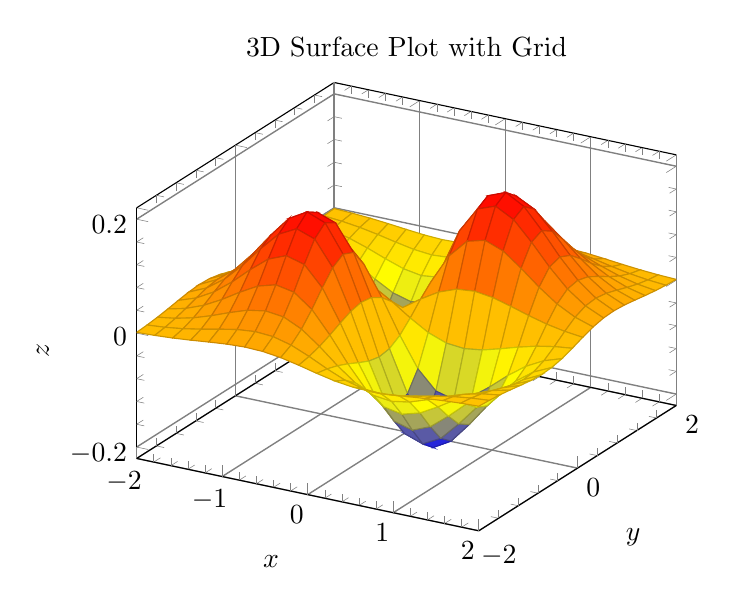
\begin{tikzpicture}
    \begin{axis}[
        title=3D Surface Plot with Grid,
        xlabel=$x$,
        ylabel=$y$,
        zlabel=$z$,
        grid=major, % Enables major grid lines
        % Optional: Customize grid appearance
        major grid style={gray,line width=0.5pt},
        minor tick num=4, % Number of minor ticks between major ticks
        minor grid style={lightgray,dotted},
        view={30}{30}, % Sets the viewing angle (azimuth, elevation)
        domain=-2:2, % x-domain
        y domain=-2:2, % y-domain
        samples=20, % Number of samples for the plot
        % colormap/jet, % Sets the color map
        % colormap/PiYG,
        % colorbar,
        % colorbar style={
        %     title=Color key,
        %     ylabel=Z-value,
        %     ytick={-.2,-0.1,...,.2},
        %     yticklabel style={
        %         text width=2.5em,
        %         align=right,
        %         /pgf/number format/.cd,
        %             fixed,
        %             fixed zerofill
        %     }
        % }
    ]
        \addplot3[
            surf, % Creates a surface plot
            % shader=faceted interp, 
            % shader= interp,
            % draw opacity=0.1,
            % fill opacity=0.3,
        ] {x*y*exp(-x^2 - y^2)}; % The function to plot

        % \node[rotate=45] at (axis cs:1,-1,0) {{\color{white}Ditch}};
    \end{axis}
\end{tikzpicture}

\end{document}